\documentclass{minimal}

\usepackage{amsmath}
\usepackage{calc}
\usepackage{tikz}
\usetikzlibrary{arrows,shapes,decorations,positioning,
				decorations.pathmorphing,decorations.pathreplacing,
				automata,backgrounds,
				petri,topaths,trees,
				fit,circuits.ee.IEC}	%To use diverse features from tikz		

\begin{document}

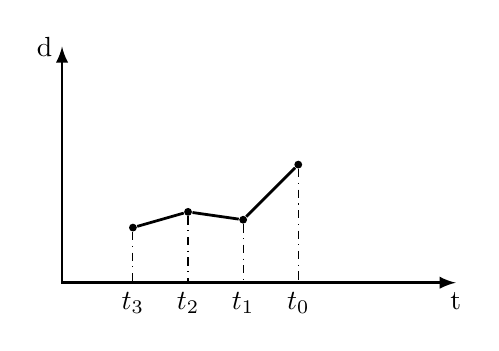
\begin{tikzpicture}

	\node[anchor=east] (d) at (0,3) {d};
	\node[anchor=north] (t) at (5,0) {t};
	\draw[latex-latex,line width=1pt] (d.east)-- (0,0) -- (t.north);

	\coordinate[fill,circle,inner sep=1pt] (d3) at (0.9,0.7);
	\coordinate[fill,circle,inner sep=1pt] (d2) at (1.6,0.9);
	\coordinate[fill,circle,inner sep=1pt] (d1) at (2.3,0.8);
	\coordinate[fill,circle,inner sep=1pt] (d0) at (3,1.5);

	%\coordinate[fill,circle,inner sep=1pt] (dnext1) at (4,2.5);
	%\coordinate[fill,circle,inner sep=1pt] (dnext2) at (4,2.12);

	%\coordinate[] (dprev2) at (2.3,1.067);

	\draw[black,line width=1pt] (d3) -- (d2) -- (d1) -- (d0);
	%\draw[red,line width=1pt] (d0) -- (dnext1);
	%	\draw[red,line width=0.7pt,dashed] (d1) -- (d0);
	%\draw[blue,line width=1pt] (d0) -- (dnext2);
	%	\draw[blue,line width=0.7pt,dashed] (dprev2) -- (d0);

	\node[anchor=north] (t3) at (0.9,0) {$t_3$};
	\node[anchor=north] (t2) at (1.6,0) {$t_2$};
	\node[anchor=north] (t1) at (2.3,0) {$t_1$};
	\node[anchor=north] (t0) at (3,0) {$t_0$};
	%\node[anchor=north] (tnext) at (4,0) {$t_{next}$};
	\draw[dashdotted] (d3) -- (t3);
	\draw[dashdotted] (d2) -- (t2);
	\draw[dashdotted] (d1) -- (t1);
	\draw[dashdotted] (d0) -- (t0);
	%\draw[dashdotted] (dnext1) -- (tnext);

\end{tikzpicture}

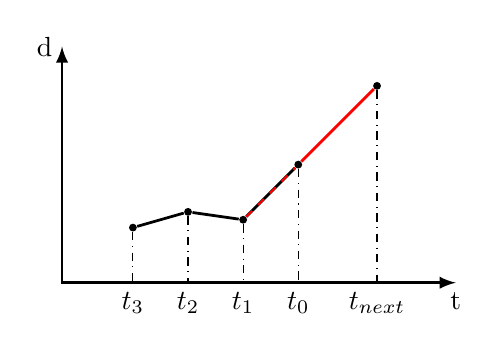
\begin{tikzpicture}

	\node[anchor=east] (d) at (0,3) {d};
	\node[anchor=north] (t) at (5,0) {t};
	\draw[latex-latex,line width=1pt] (d.east)-- (0,0) -- (t.north);

	\coordinate[fill,circle,inner sep=1pt] (d3) at (0.9,0.7);
	\coordinate[fill,circle,inner sep=1pt] (d2) at (1.6,0.9);
	\coordinate[fill,circle,inner sep=1pt] (d1) at (2.3,0.8);
	\coordinate[fill,circle,inner sep=1pt] (d0) at (3,1.5);

	\coordinate[fill,circle,inner sep=1pt] (dnext1) at (4,2.5);
	%\coordinate[fill,circle,inner sep=1pt] (dnext2) at (4,2.12);

	%\coordinate[] (dprev2) at (2.3,1.067);

	\draw[black,line width=1pt] (d3) -- (d2) -- (d1) -- (d0);
	\draw[red,line width=1pt] (d0) -- (dnext1);
		\draw[red,line width=0.7pt,dashed] (d1) -- (d0);
	%\draw[blue,line width=1pt] (d0) -- (dnext2);
	%	\draw[blue,line width=0.7pt,dashed] (dprev2) -- (d0);

	\node[anchor=north] (t3) at (0.9,0) {$t_3$};
	\node[anchor=north] (t2) at (1.6,0) {$t_2$};
	\node[anchor=north] (t1) at (2.3,0) {$t_1$};
	\node[anchor=north] (t0) at (3,0) {$t_0$};
	\node[anchor=north] (tnext) at (4,0) {$t_{next}$};
	\draw[dashdotted] (d3) -- (t3);
	\draw[dashdotted] (d2) -- (t2);
	\draw[dashdotted] (d1) -- (t1);
	\draw[dashdotted] (d0) -- (t0);
	\draw[dashdotted] (dnext1) -- (tnext);

\end{tikzpicture}

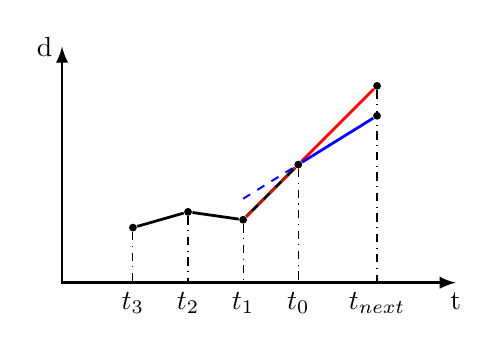
\begin{tikzpicture}

	\node[anchor=east] (d) at (0,3) {d};
	\node[anchor=north] (t) at (5,0) {t};
	\draw[latex-latex,line width=1pt] (d.east)-- (0,0) -- (t.north);

	\coordinate[fill,circle,inner sep=1pt] (d3) at (0.9,0.7);
	\coordinate[fill,circle,inner sep=1pt] (d2) at (1.6,0.9);
	\coordinate[fill,circle,inner sep=1pt] (d1) at (2.3,0.8);
	\coordinate[fill,circle,inner sep=1pt] (d0) at (3,1.5);

	\coordinate[fill,circle,inner sep=1pt] (dnext1) at (4,2.5);
	\coordinate[fill,circle,inner sep=1pt] (dnext2) at (4,2.12);

	\coordinate[] (dprev2) at (2.3,1.067);

	\draw[black,line width=1pt] (d3) -- (d2) -- (d1) -- (d0);
	\draw[red,line width=1pt] (d0) -- (dnext1);
		\draw[red,line width=0.7pt,dashed] (d1) -- (d0);
	\draw[blue,line width=1pt] (d0) -- (dnext2);
		\draw[blue,line width=0.7pt,dashed] (dprev2) -- (d0);

	\node[anchor=north] (t3) at (0.9,0) {$t_3$};
	\node[anchor=north] (t2) at (1.6,0) {$t_2$};
	\node[anchor=north] (t1) at (2.3,0) {$t_1$};
	\node[anchor=north] (t0) at (3,0) {$t_0$};
	\node[anchor=north] (tnext) at (4,0) {$t_{next}$};
	\draw[dashdotted] (d3) -- (t3);
	\draw[dashdotted] (d2) -- (t2);
	\draw[dashdotted] (d1) -- (t1);
	\draw[dashdotted] (d0) -- (t0);
	\draw[dashdotted] (dnext1) -- (tnext);

\end{tikzpicture}

\end{document}
